\documentclass[12pt, a4]{article} % article for short, book for long [thesis]
%\documentclass[12pt, a4, twocolumn]{book} %split columns

\usepackage{graphicx} % support the \includegraphics command and options
\graphicspath{{../Images/}}
\usepackage{listings} %lslisting for code snippets
\usepackage{color} %colouring code in lstlisting
\usepackage{hyperref} %hyper-links when referencing
\usepackage[export]{adjustbox} %for figure alignment
\usepackage[a4paper, left=2cm, right=2cm, top=2.5cm, bottom=3cm]{geometry} %for setting page margin.
\usepackage{wrapfig} %wrapping text around figure
\usepackage{paracol} %splitting page parallel
\usepackage{amsmath} %maths equations
\usepackage[font=small,labelfont=bf]{caption} %changing caption font size
\usepackage{multirow} %multirow tables
\usepackage{adjustbox,lipsum} %setting table size
\usepackage{mathtools} %multivalue functions
\usepackage[colorinlistoftodos]{todonotes} %Todo notes/comments


\definecolor{dkgreen}{rgb}{0,0.6,0}
\definecolor{gray}{rgb}{0.5,0.5,0.5}
\definecolor{mauve}{rgb}{0.58,0,0.82}

\lstset{frame=tb,
  language=Python,
  aboveskip=3mm,
  belowskip=3mm,
  showstringspaces=false,
  columns=flexible,
  basicstyle={\small\ttfamily},
  numbers=none,
  numberstyle=\tiny\color{gray},
  keywordstyle=\color{blue},
  commentstyle=\color{dkgreen},
  stringstyle=\color{mauve},
  breaklines=true,
  breakatwhitespace=true,
  tabsize=3
}

\setlength\parindent{0pt} 
\usepackage[utf8]{inputenc}
\usepackage[english]{babel}
\usepackage[nottoc]{tocbibind}



\hypersetup{pageanchor=false}

\begin{document}
\onecolumn


\thispagestyle{empty}
\begin{center}

\begin{figure}[h!]
    \centering
    
\includegraphics[width=\linewidth]{Trinity Logo.jpg}
\end{figure}

\noindent\makebox[\linewidth]{\centering \rule{.7\paperwidth}{0.4pt}} \\
\vspace{.4cm} 
\Large \textbf{Song recommendations using Spotify API}  \\
\vspace{.5cm}

Shane Keane, Dylan Kierans, Alexander Sanfilippo \\17329836, 21346261, 21343904\\
\vspace{.4cm}
\textbf{ CS7CS4 Machine Learning Group Project} \\
\vspace{.4cm} 
\noindent\makebox[\linewidth]{\centering \rule{.7\paperwidth}{0.4pt}}
\end{center}

\tableofcontents

\newpage
\section*{Introduction [half page]}
Streaming platforms are as popular as ever. While the film/TV and podcast streaming sector has seen an increase in competition in recent years, the same can not be said for music platforms. Spotify is the home of music streaming. We take a slight turn away from user-specific recommender systems which the platform is well known for, and instead look at automating the classification of songs into genre-specific playlists. This would be a useful tool for a growing resource such as Spotify. The music platform was founded in 2008, and now contains \href{https://newsroom.spotify.com/company-info/}{over 70 million songs}. That is an average of about 14,000 songs per day since launch, with Spotify reporting earlier this year that they now 'publish' over \href{https://www.youtube.com/watch?v=Vvo-2MrSgFE&ab_channel=Spotify}{60,000 songs per year }. \newline

That's a lot of songs to tag, and its likely Spotify already have advanced deep learning software analysing every part of the platform and user interaction. We hope to imitate a possible genre classification model the multi-billion company may use.


\section{Dataset and Features [1 page]}
\subsection{Data Collection}

Spotify provide a free API for developers [https://developer.spotify.com/documentation/web-api/], which we use for data collection in order to compare songs . Spotify stores a whole range of metadata which is accessible via its API such as information about artists, users, podcasts and can be used to return search queries for 3rd party applications. For our project we are just interesting in playlist and song information. In particular, gathering the audio feature attributes of every song in specific playlists.

The project sets out to use these audio features as the input parameters (including feature engineering if necessary) to create an effective multi-class classification model. Features of interest include normalized parameters {acousticness, danceability, energy, instrumentalness, liveness, speechiness, valence}. Other features which aren't normalized but may be of interest include continuous {duration, tempo}, and discrete { key, mode, time signature}


\subsection{Training Data}
We chose 8 genre-specific spotify playlists each with over 200 songs, to train our models. The genres we chose to work with are:
\begin{itemize}
\item Jazz
\item Country/folk
\item Classical
\item Hip Hop
\item Rock
\item Kpop
\item Heavy Metal
\item Dance
\end{itemize}


Of course music genre isn't entirely objective, so it is expected that there will be noise in training data, and it won't be possible to create a 100\% accurate model. In any case, we had a total of 2300 songs and were left with 2276 after removing duplicates. For each of these songs we gathered all audio features from the API. We then added an additional column to each dataset specifying which playlist number we had got the song from. We now had 2276 input vectors, and a set of 8 possible target values to train the model on.\newline

In order to test models, we perform a 5-fold train/test data split.\newline

\todo[inline]{Comment on not just evaluating model, but also evaluating how explanatory the audio features are}

\section{Methods [1 page]}
Our goal was to create an accurate multi-class classification model for a finite number of genres. For the sake of simplicity, and in order to gain an understanding of the audio features from Spotify, we work on just taking the most likely classification from the model predictions. We understand that more complex measures of accuracy can be considered by taking a more dynamic approach to accepting multiple-classes within a certain threshold. In an industry application of such a model this would be a useful consideration.\newline 

However, for the purpose of this project we focused on running a wide variety of models in order to find the one which best captured the behaviour of the data.


\todo[inline] {List all our models from most basic $->$ most complex.}
\todo[inline] {Comment on pipelining method for normalizing data}

\subsection{Some baseline models}
\subsection{kNN}
\subsection{Logistic regression based models}
\subsection{MLP}
A multi-layer perceptron (MLP) is a machine learning algorithm that uses an architecture known as a "neural network" to create a function between the feature(s) and
target(s) of the training data.  In the simplest case, the model has 3 layers: an input layer of the features, an output layer of the targets, and a "hidden" layer in-between.  A "node" exists for each feature and target in the input and output layers respectively, whereas a hidden layer's number of nodes is a hyper-parameter determined by the model's creator.  These nodes can be thought of as being like neurons in a living brain, thus the name "neural network".  Between two given layers, a parameter or "weight" exists for each possible path between the nodes.  For example, if layer n has 4 nodes and layer n+1 has 5, there will be 20 parameters in total between these two layers.  These parameters are used to form linear equations: For a given node in layer n+1, its value is a \[f(\theta_0X1 + \theta_1X2 + \cdots + \theta_5X5)\], where \(X1\cdotsX5\) are the values of the nodes in layer n, and the\(\theta\)'s are the parameters.  This linear equation is then passed to an activation function \(f()\), which is vital to the back-propagation phase which relies on stochastic gradient descent.  To train the parameters of an MLP, first the a vector of training data features are sent to the input layer, and the nodes of the next (hidden) layer are calculated.  In the last layer an output function \(g()\) (for example, the sigmoid function) processes the linear equation from the previous layer's weights and values, and produces the predicted target(s) \(hat{y}\). This part of the process is known as "forward propagation".  In the aforementioned back-propagation stage, the difference between \(hat{y}\) and \(y^{(i)}\) (the target from the training data for the corresponding features \(x^{(i)}\)) is calculated. This error information is sent backwards through the network, allowing each weight to be adjusted.  Thus, over many epochs (an epoch being being a single pass of all the training data through the network for forward and back propagation) the model "learns" to better predict the targets.   
\section{Experiments/Results/Discussion [2-3 pages]}
For the MLP model the parameters to be trained were the weights between the layers.  The hyperparameters are the number of nodes in the hidden layer(s), the value of the L2 regularization coefficient C, and the number of hidden layers over which to divide the number of nodes in the hidden layers.  The number of nodes in the hidden layers can have a huge effect on performance, but increasing the number can result in long training times and overfitting, so we decided to perform cross-validation for this value.  The value of the coefficient C can also greatly effect accuracy, as Iwehad seen in previous model training, so it too had to be cross-validated.  The number of layers was a bit of an afterthought, since we did not even know at first that you could have multiple layers with sklearns MLPClassfier, bit having seen what effect model depth could have in CNNs, we decided to cross evaulate it as well.  We used 5-folds for all of these, and accuracy was used as the main metric. The AUC was also calculated for comparison.  Initial tests triggered a warning from sklearn that the model was not converging before the max number of iterations was reached, so this variable was increased to 10000 for the remaining tests.  First, for cross-validating the number of hidden layers, we ran this cross validation and a few values of "C", and the following plots show the results: 

\begin{figure}[h]
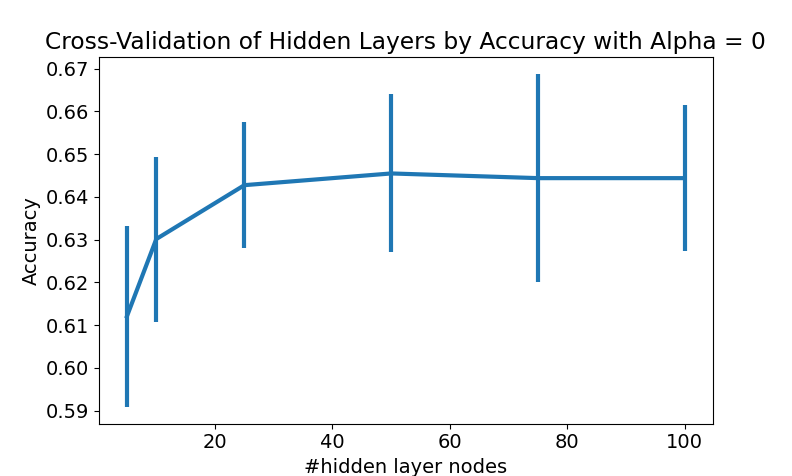
\includegraphics[width=8cm]{crossValLayers3[newData,acc,A0].png}
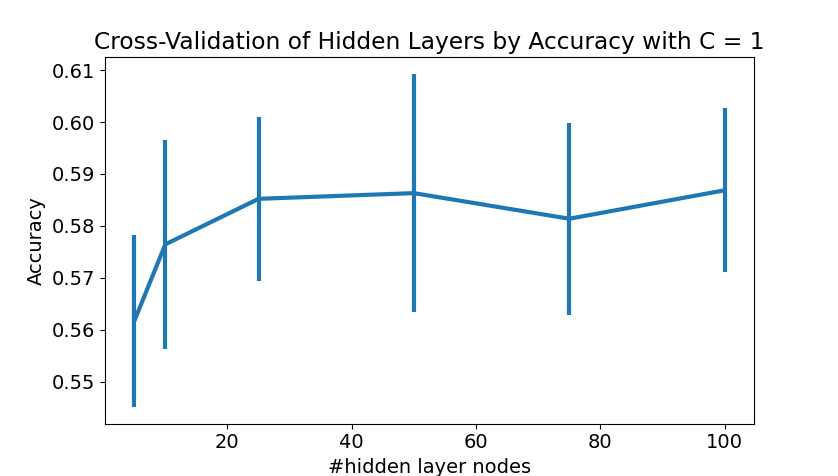
\includegraphics[width=8cm]{crossValLayers3[newData,acc,C1].png}
\end{figure}
\begin{figure}[h]
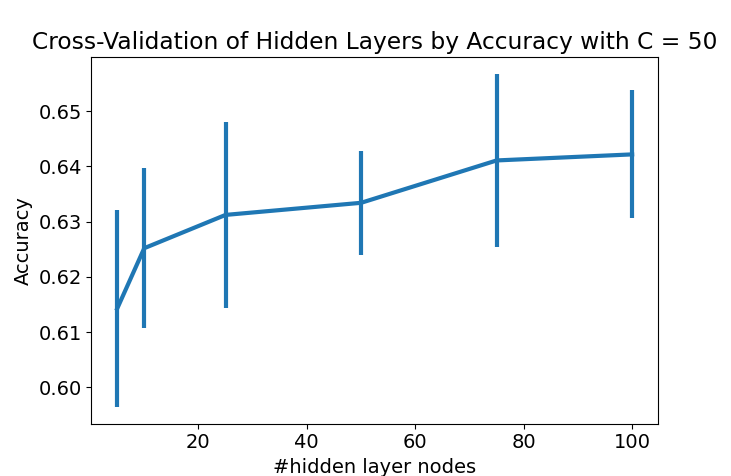
\includegraphics[width=8cm]{crossValLayers3[newData,acc,C50].png}
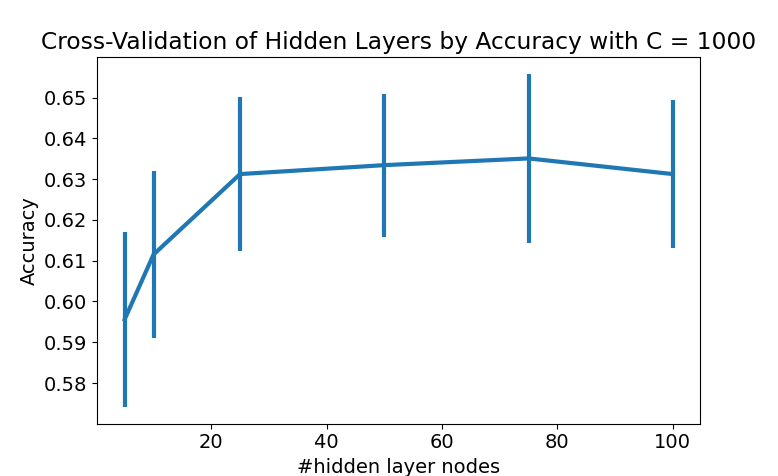
\includegraphics[width=8cm]{crossValLayers3[newData,acc,C1000].png}
\end{figure}
In general the accuracy increases as the number of nodes in the hidden layer increases, however there is little to no value beyond 50 neurons, so this value was selected moving forward.  Furthermore, the accuracy was best with a C value of 1000, so this value was selected as well.  Finally, cross-validation on the number of hidden layers was performed: 

\begin{figure}[h]
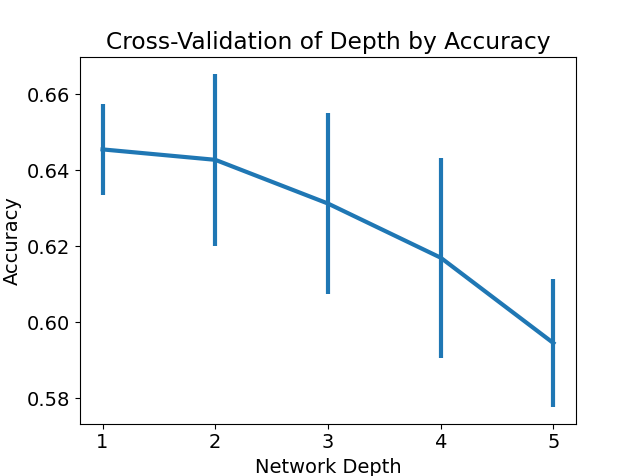
\includegraphics[width=8cm]{Cross-Val Depth.png}
\end{figure}

This plot shows that as we divide up the 50 nodes in the one hidden layer into separate layers (increases the "depth" of the neural network), there is a noticeable decrease
in accuracy.  Thus, just 1 layer of 50 nodes was selected based off this evidence.  Next we will look at the results of the model using these hyperparameters.  
\begin{figure}[h]
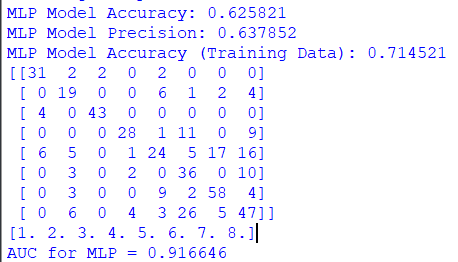
\includegraphics[width=8cm]{outputMLP.png}
\end{figure}
The ultimate accuracy of the MLP model was about 64\% (plus or minus 1\%) on the training data, with an accuracy of over 71\% on the testing data.  This discrepancy between the training and testing data accuracy suggests some overfitting is occurring.  This means that the model is training well on the training data, but is not generalizing as well.  The accuracy of the baseline "cosine similarity" model is 0.33, so the MLP model performs significantly better than the baseline.  Creating ROC curves for this model was difficult, since it is a multi-class situation, but the AUC could be calculated using the roc\_auc\_score() method.  Using the parameter values 'ovr' and 'macro', this method compares each class to each other when calculating true/false positives and negatives, and then finds the average.  An AUC of ~.92 suggests a favorable ratio of true-positives to false positives.    
\section{Summary [100-200 words]}
\section{Contributions}
\section{Github Link}








\end{document}
